\documentclass{beamer}

\title{Brancher AnyBlok à 14 ans d'historique métier}
\subtitle{Une histoire terrifiante de PHP, MySQL et MsSQL}
\author{Jean-Sébastien SUZANNE et Hugo QUEZADA}
\date{2 novembre 2019}

\newcommand{\TwitterLogo}{\protect
\includegraphics[height=
1.7ex,keepaspectratio]{./twitter.png}}
\newcommand{\EmailLogo}{\protect
\includegraphics[height=
1.7ex,keepaspectratio]{./email.png}}
\newcommand{\AnyBlokLogo}{\protect
\includegraphics[height=
1.7ex,keepaspectratio]{./anyblok.png}}

\usetheme{Amsterdam}
\begin{document}
	\frame {
		\titlepage
	}
	
	\frame {
		\frametitle{Qui sommes nous ?}
		
		\begin{columns}
            \begin{column}{3cm}
                Logo Sensee
			\end{column}
			\begin{column}{3cm}
				Logo LMC
			\end{column}
		\end{columns}
			
		\hfill \break			
		\begin{columns}
            \begin{column}{5cm}
                \textbf{\AnyBlokLogo{} Sébastien Suzanne}
		    	\begin{itemize}
			  		\item Répond aussi au nom de PAPABLOK
			  		\item \TwitterLogo{} @jssuzanne
			    	\item \EmailLogo{} js.suzanne@sensee.com
		    	\end{itemize}
			\end{column}
			\begin{column}{5cm}
				\textbf{Hugo Quezada}
		    	\begin{itemize}
			  		\item Dis le petit Basque du Chili
			  		\break
			    	\item \EmailLogo{} h.quezada@sensee.com
		    	\end{itemize}
			\end{column}
		\end{columns}
	}
	
	\frame{
		\frametitle{Existant}
		\framesubtitle{14 ans de code...}
		\begin{itemize}
			\pause
			\item Code legacy en PHP5 (pas de troll SVP)
			\item Pas de framework, beaucoup de code, très peu d'objet
			\break
			\pause
			\item Pas de tests
			\item Pas de CI
			\break
			\pause
			\item Pas d'ORM
		\end{itemize}
	}
	
	\frame{
		\frametitle{Existant}
		\framesubtitle{Une BdD un peu complexe...}
		\begin{itemize}
			\item  Schémas de base de données multiples
			\pause
			\item  Écosystème avec plusieurs SGBD (MySQL, MsSQL) souvent sans API
			\begin{figure}[p]
				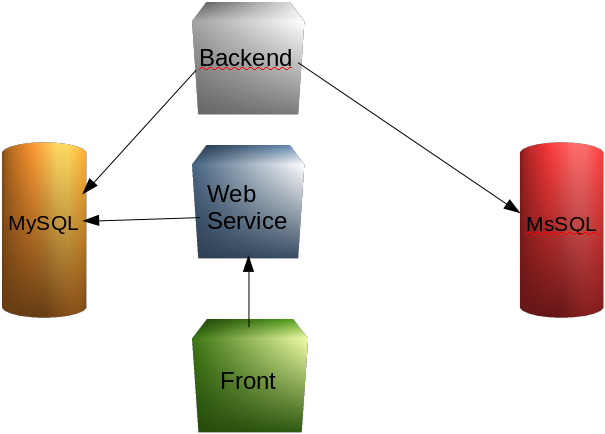
\includegraphics[height=25ex,keepaspectratio]{./schema_simplifie_lmc.png}
				\caption{Schéma simplifié}
			\end{figure}
		\end{itemize}
	}
	
	\frame{
		\frametitle{Vision finale}
		\framesubtitle{L'objectif}
		\begin{itemize}
		    \item Un code python propre et testé
			\item Une API simple et uniforme, utilisé dans tous nos projets
			\item Une application plus proche des standards actuels
			\item Un projet plus séduisant et plus attrayant pour des potentiels futurs développeurs 
		\end{itemize}
	}
	\frame{
		\frametitle{Vision finale}
		\framesubtitle{La stratégie}
		\begin{itemize}
			\item Modèle d'étranglement (Strangle pattern)
			\begin{figure}[p]
				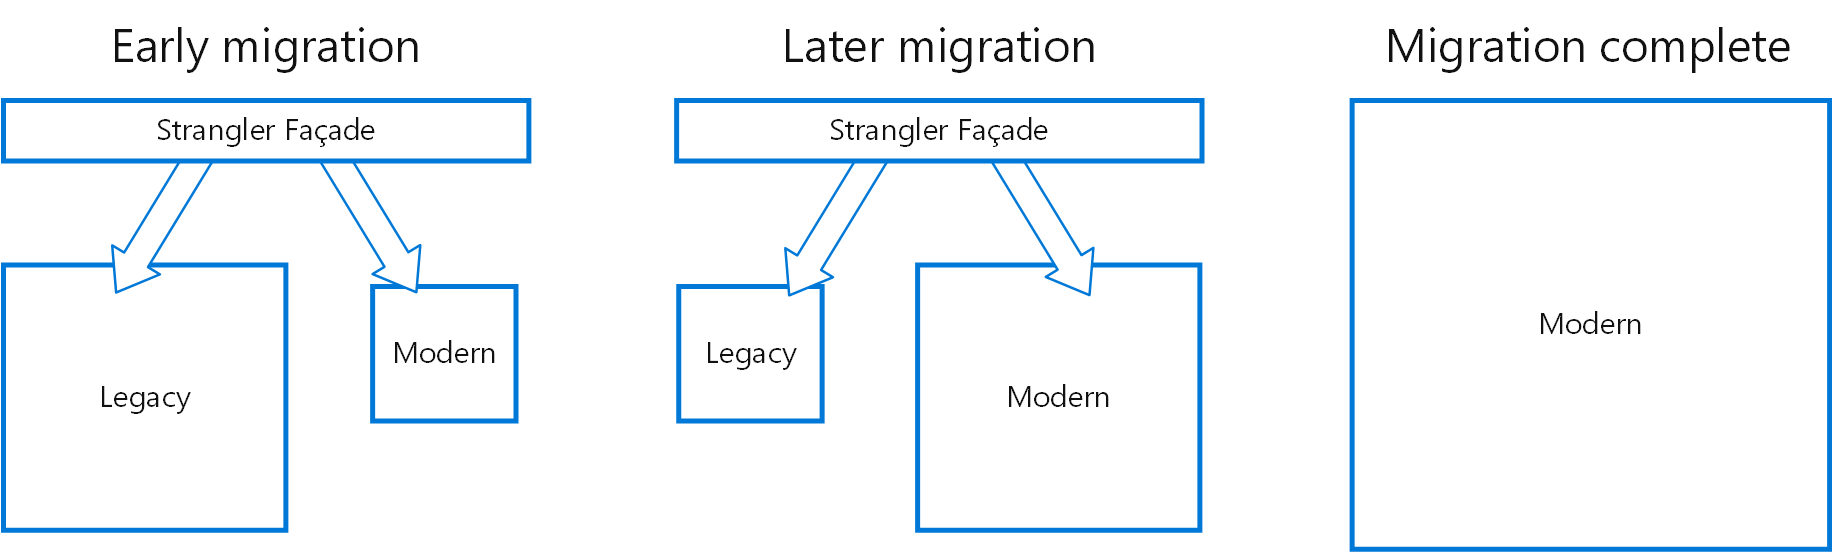
\includegraphics[height=15ex,keepaspectratio]{./strangler.png}
			\end{figure}
			\item Mapping des tables avec un nommage plus clair
			\item Développement piloté par les tests (TDD)
		\end{itemize}
	}
	\frame{
		\frametitle{Pourquoi avoir choisi AnyBlok ?}
		\framesubtitle{AnyBlok: Présentation}
	}
	\frame{
		\frametitle{Pourquoi avoir choisi AnyBlok ?}
		\framesubtitle{AnyBlok: Écrire des tests pour notre Model}
	}
	\frame{
		\frametitle{Pourquoi avoir choisi AnyBlok ?}
		\framesubtitle{AnyBlok: Définir le Model}
	}
	\frame{
		\frametitle{Pourquoi avoir choisi AnyBlok ?}
		\framesubtitle{AnyBlok: Définir un Model sur une table existante}
	}
	\frame{
		\frametitle{Pourquoi avoir choisi AnyBlok ?}
		\framesubtitle{AnyBlok: Créer API web et tests unitaires associés}
	}
	\frame{
		\frametitle{Pourquoi avoir choisi AnyBlok ?}
		\framesubtitle{AnyBlok: Créer un console script dédié par service}
	}
	\frame{
		\frametitle{Evolutions et intégrations dans AnyBlok}
		\framesubtitle{Compatibilité avec plusieurs SGBD}
		\begin{itemize}
			\item Commits implicites pour les tests unitaires
			\item Datetime sans time zone
			\item Contraintes exclusives à PostgreSQL
			\item Options par défaut pour MySQL (innodb, mode transactionnel)
			\item Cas des champs JSON
		\end{itemize}
	}
	\frame{
		\frametitle{Evolutions et intégrations dans AnyBlok}
		\framesubtitle{Définition de schémas par modèle ou par namespace}
		\begin{itemize}
			\item Apporter plus de cohérence avec la BdD.
			\item Utilisation de suffixes ou préfixes pour les schémas
			\begin{itemize}
				\item Initialisation de schémas vides pour lancer les tests unitaires.
			\end{itemize}
		\end{itemize}
	}
	\frame{
		\frametitle{Fin}
		\begin{columns}
			\begin{column}{4cm}
			\end{column}
			\begin{column}{8cm}
				Des questions ? 
				\break
				Des remarques ?
			\end{column}
		\end{columns}
	}
		
\end{document}
